
\chapter{Langage des expressions arithmétiques}

	\section{Syntaxe}

Nous pouvons formaliser la syntaxe de notre langage arithmétique grâce à la notation BNF : \\
$E_A$ ::= $n$ $|$ $x$ $|$ $E_A$ + $E_A$ $|$ $E_A$ - $E_A$ $|$ $E_A$ $\times$ $E_A$ $|$ $E_A$ / $E_A$ 
\vspace{1\baselineskip} \\
Un formalisme classiquement utilisé est d'écrire un système d'inférence : \\
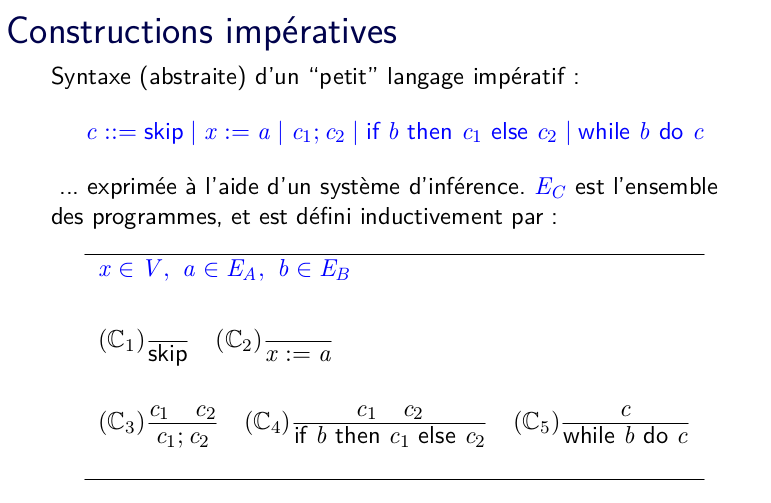
\includegraphics[height=4cm]{\Arithroot/definition_inductive.png}
Cela revient à écrire un type inductif, ou une définition inductive. C'est ce que nous verrons lorsque nous écrirons cette syntaxe dans Coq ou dans Dedukti.

	\subsection{Traduction en OCaml}
	\lstinputlisting[language=OCaml, linerange={10-16}]{\OCamlroot/OCaml_exemple.ml}
	
	\subsection{Traduction en K}
	\lstinputlisting[language=K, linerange={1-11}]{\Kroot/K_exemple.k}

	\subsection{Traduction en Coq}
	\subsection{Traduction en Dedukti}


\section{Sémantique dénotationnelle}
Nous cherchons ici à interpréter des expressions arithmétiques, c'est-à-dire donner, à chaque expression arithmétique, une valeur appartenant à $\mathbb{V} = \mathbb{Z} \cup \{ Err \}$, où $Err$ dénote une erreur lors de l’interprétation.

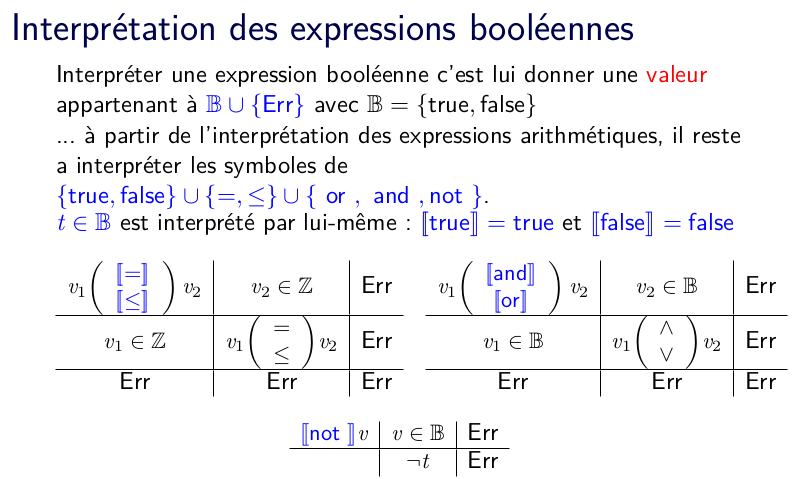
\includegraphics[height=5cm]{\Arithroot/interpretation.png}

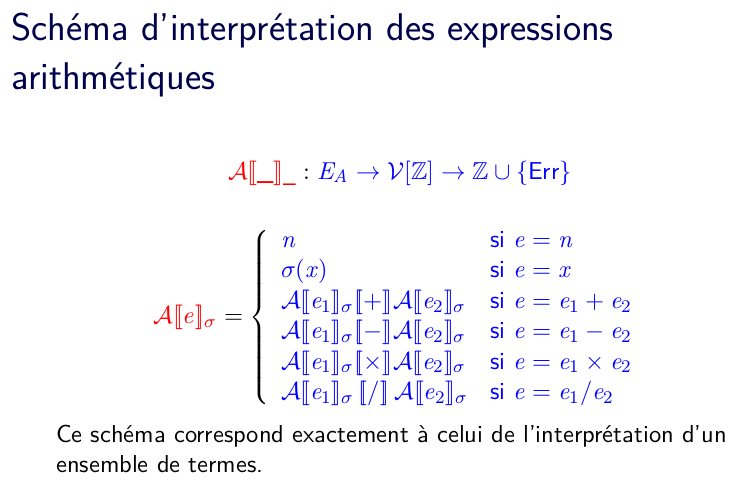
\includegraphics[height=5cm]{\Arithroot/schema_interpretation.png}

	\subsection{Traduction en OCaml}
Nous commençons d'abord par définir le type des valeurs possibles attendues ainsi que celui des valuations :
\lstinputlisting[language=OCaml, linerange={22-26}]{\OCamlroot/OCaml_exemple.ml}
Ensuite, nous définissons l'interprétation de chacun des opérateurs arithmétiques :
\lstinputlisting[language=OCaml, linerange={39-41,54-56,65-67,77-79}]{\OCamlroot/OCaml_exemple.ml}
Enfin, nous en déduisons l'évaluation de ces opérateurs :
\lstinputlisting[language=OCaml, linerange={91-97}]{\OCamlroot/OCaml_exemple.ml}

	\subsection{Traduction en K}
\lstinputlisting[language=K, linerange={13-39}]{\Kroot/K_exemple.k}

	\subsection{Traduction en Coq}
	\subsection{Traduction en Dedukti}

%\lstinputlisting[language=OCaml, linerange={137-142}]{\OCamlroot/OCaml_exemple.ml}

%\lstinputlisting[language=OCaml, linerange={157-173}]{\OCamlroot/OCaml_exemple.ml}

%\lstinputlisting[language=OCaml, linerange={220-225}]{\OCamlroot/OCaml_exemple.ml}
















\section{Sémantique opérationnelle d’évaluation à grands pas}

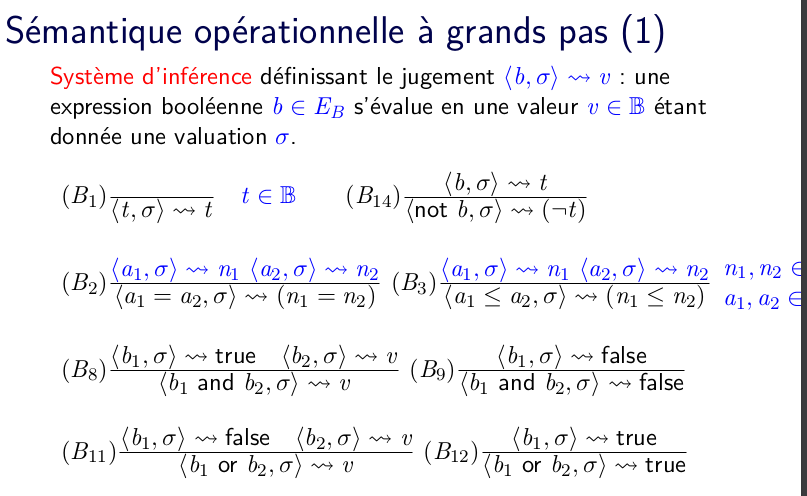
\includegraphics[height=5cm]{\Arithroot/eval_grands_pas.png}

Déterminisme \\
Proposition : \\
%∀a ∈ E A ∀σ ∈ V[Z] ∀v 1 , v 2 ∈ VA
%(ha, σi
%v 1 et ha, σi
%v 2 ) ⇒ v 1 = v 2
%Preuve : Par induction sur a.



Équivalence des sémantiques opérationnelle et
dénotationnelle

Propriétés Évaluation des expressions arithmétiques : variables

Expressions arithmétiques équivalentes (1) \\
Caractériser les expressions arithmétiques qui s’évaluent à la même valeur.
%a 1 ∼ a 2 ⇔ (∀v ∈ VA ∀σ ∈ V[Z] ha 1 , σi
%v ⇔ ha 2 , σi v)
%Proposition : $∼$ est une congruence. \\



\section{Sémantique opérationnelle d’évaluation à petits pas}

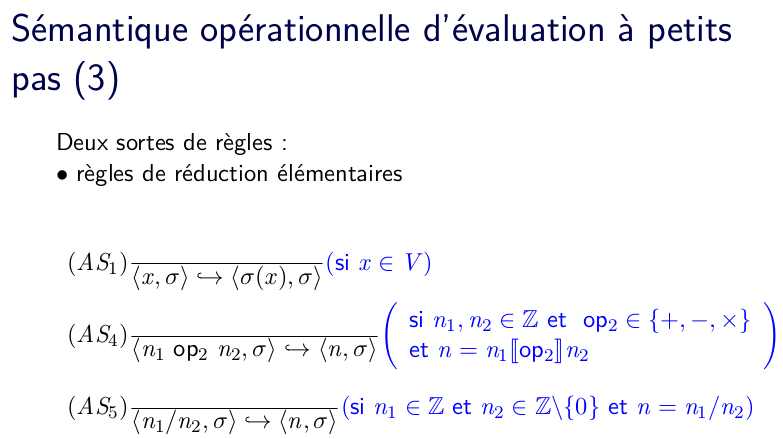
\includegraphics[height=5cm]{\Arithroot/eval_petits_pas_1.png}

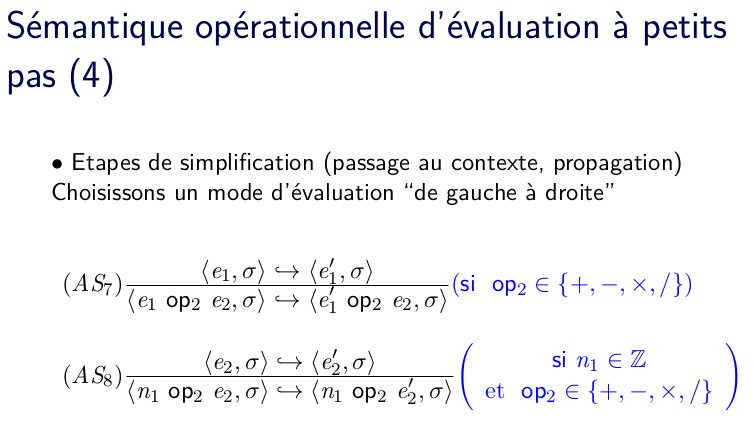
\includegraphics[height=5cm]{\Arithroot/eval_petits_pas_2.png}

déterministe


\section{Autre présentation : Contexte d'évaluation}

Cette autre présentation plus synthétique a été proposée par Andrew Wright et Matthias Felleisen.
Toutes les règles de simplification précédentes sont réduites à une seule : la règle de passage au contexte. \\

Cette présentation a été préférée lors de notre modélisation avec K :

\lstinputlisting[language=K, linerange={28-39}]{\Kroot/K_exemple.k}


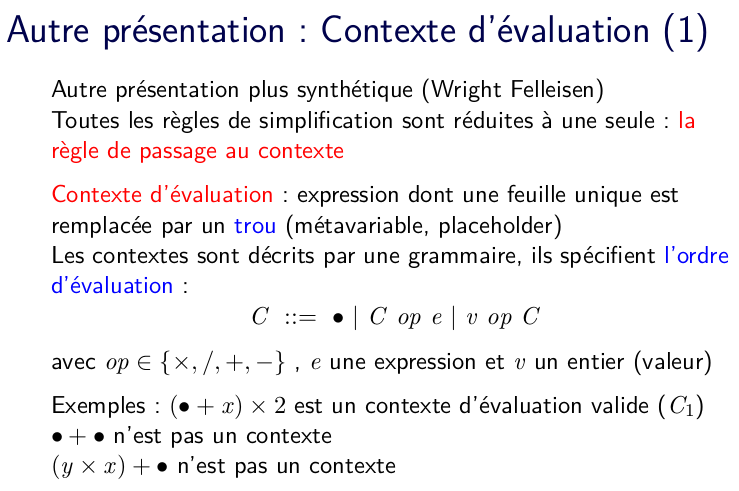
\includegraphics[height=5cm]{\Arithroot/contexte_eval_1.png}

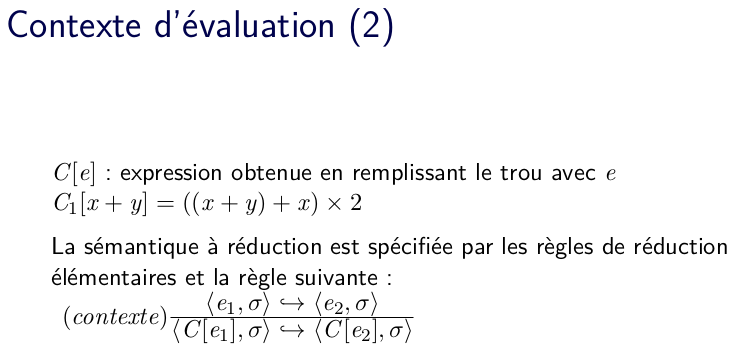
\includegraphics[height=5cm]{\Arithroot/contexte_eval_2.png}

Équivalence des sémantiques ?

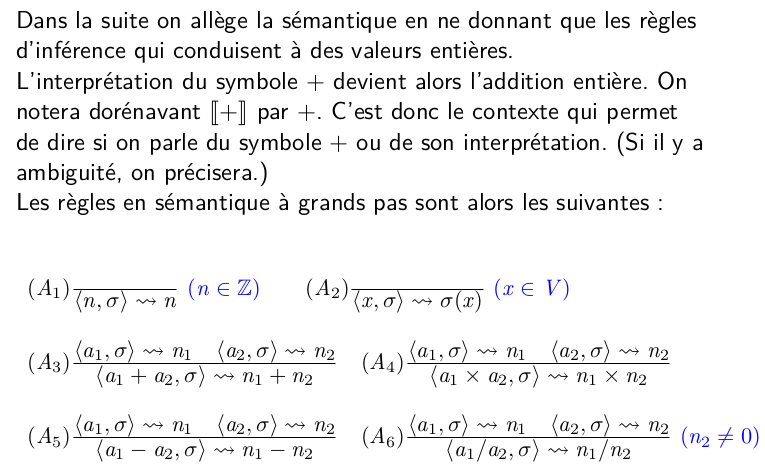
\includegraphics[height=5cm]{\Arithroot/simplification_notations.png}